\documentclass{beamer}
\usepackage[utf8]{inputenc}
\usepackage[T1]{fontenc}
\usepackage{graphicx}
\usepackage{tcolorbox}
\usepackage{hyperref}
\hypersetup{
    colorlinks=true,
    linkcolor=pink,
    urlcolor=cyan,
    urlbordercolor=cyan,
}
\graphicspath{ {./images/} }

\usetheme{Arguelles}

\title{Tutorial 6}
\subtitle{CS3241 Computer Graphics (AY23/24)}
\date{\today}
\author{Wong Pei Xian}
\institute[]{\email{e0389023@u.nus.edu}}

\begin{document}

\frame[plain]{\titlepage}

\section{Question 1}

\begin{frame}
    \frametitle{Question 1}

    % \begin{tcolorbox}[colback=teal!5!white] \textcolor{teal}{pollev.com/peixian} \end{tcolorbox}
    % \vspace*{1em}

    In which pipeline stage and in which coordinate space is the OpenGL 
    \textbf{built-in lighting computation} performed? 

    \begin{tcolorbox}
        OpenGL's built-in lighting computation is performed when
        \texttt{GL\_LIGHTING} is enabled.
    \end{tcolorbox}
\end{frame}

\begin{frame}
    \frametitle{Question 1}

    \begin{itemize}
        \item vertex processing: We do calculations per vertex 
        \item camera space: We need the view direction, it's defined after camera space
    \end{itemize}
    
    \begin{center}
        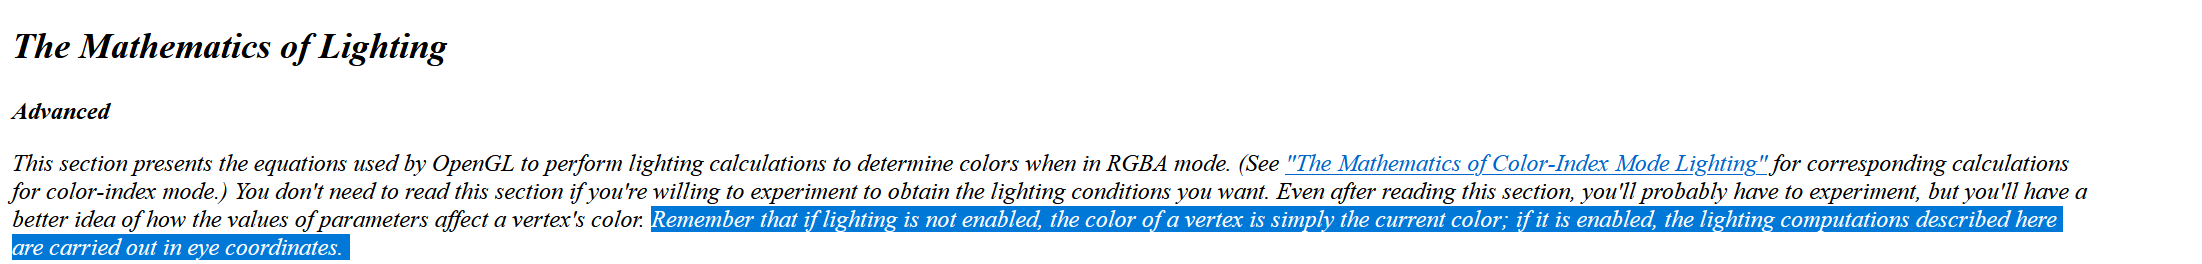
\includegraphics[scale=0.3]{q1.png}
        \small
        Reference at \hyperlink{https://www.glprogramming.com/red/chapter05.html}{RED BOOK}
    \end{center}

\end{frame}

\section{Question 2}

\begin{frame}
    \frametitle{Question 2}

    %\begin{tcolorbox}[colback=teal!5!white] \textcolor{teal}{pollev.com/peixian} \end{tcolorbox}

    We are using Phong Illumination Equation 

    \begin{equation*}
        I_\text{Phong} = I_a k_a + I_p k_d  (N \cdot L) + I_p k_s (R \cdot V)^n
    \end{equation*}

    to compute a color for vertex $v$. Given that the material at $v$ is 
    \textbf{totally diffuse}, which of the following will result in a change in computed color at $v$?

\end{frame}


\begin{frame}
    \frametitle{Which will result in change of color of a diffuse material?}

    \begin{equation*}
        I_\text{Phong} = I_a k_a + I_p k_d  (N \cdot L) + I_p k_s (R \cdot V)^n
    \end{equation*}

    \begin{enumerate}
        \item Moving the light source further away from $v$, while maintaining the direction $L$.
        \item Moving the light source to a different direction from $v$, while maintaining its distance from $v$.
        \item Moving the viewpoint to a different direction from $v$.
        \item Rotating the normal vector $N$.
    \end{enumerate}

\end{frame}

\begin{frame}
    \frametitle{Which will result in change of color of a diffuse material?}

    \begin{equation*}
        I_\text{Phong} = I_a k_a + \textcolor{blue}{I_p k_d  (N \cdot L)} + I_p k_s (R \cdot V)^n
    \end{equation*}

    \begin{enumerate}
        \item Moving the light source further away from $v$, while maintaining the direction $L$. \textcolor{red}{False. No values changed}
        \item Moving the light source to a different direction from $v$, while maintaining its distance from $v$. \textcolor{teal}{True. Changes $L$}
        \item Moving the viewpoint to a different direction from $v$. \textcolor{red}{False. Changes $V$}
        \item Rotating the normal vector $N$. \textcolor{teal}{True (assuming rotating about an axis that's not itself)}
    \end{enumerate}

\end{frame}

\section{Question 3}

\begin{frame}
    \frametitle{Question 3}

    % \begin{tcolorbox}[colback=teal!5!white] \textcolor{teal}{pollev.com/peixian} \end{tcolorbox}
    % \vspace*{1em}

    A closed cylinder (with top and bottom caps) is approximated by 32 rectangles on its 
    smooth curved surface. 
    Each cap is represented as a fan of 32 triangles, 
    all sharing a vertex at the center of the cap. 

    \vspace*{1em}

    How many \textbf{distinct} vertex normal altogether are needed to model the cylinder?

\end{frame}

\begin{frame}
    \frametitle{Vertex Normals of a Cylinder}

    \begin{center}
        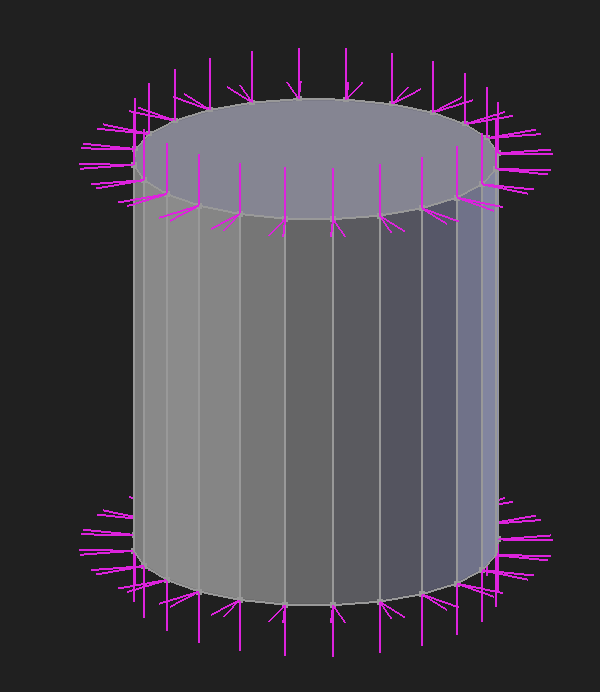
\includegraphics[scale=0.4]{images/solid_cylinder_normals.png}
    \end{center}

\end{frame}

\section{Question 4}

\begin{frame}
    \frametitle{Question 4}

    A sphere, centered at the location C, is approximated by a polygon mesh.  
    A vertex v is on the surface of the sphere, and has the location V.  
    Suppose vertex v is shared by exactly 3 polygons whose polygon normals are N1, N2, and N3.
    
    \vspace*{1em}

    Show two ways to compute the \textit{vertex normal} at v. Normalize your results to unit vectors.

\end{frame}

\begin{frame}
    \frametitle{Question 4}


    \begin{center}
        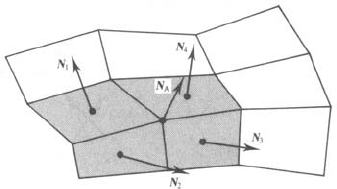
\includegraphics[scale=0.3]{q4-normalvector0.png}
        \begin{equation*}
            N_v = \frac{N_1+ N_2 + N_3}{|N_1+ N_2 + N_3|}
        \end{equation*}

        \vspace{1em}

        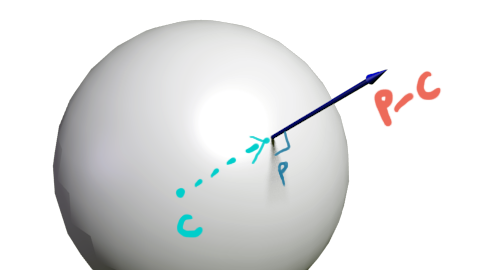
\includegraphics[scale=0.3]{q4-normalvector1.png}
        \begin{equation*}
            N_v = \frac{v - C}{|v - C|}
        \end{equation*}
    \end{center}
    
\end{frame}

\section{Question 5}

\begin{frame}
    \frametitle{Question 5}

    Find the values for $k_d, k_s, n$ to model the following:

    \begin{enumerate}
        \item Red shiny plastic (billiard ball)
        \item Dry white clay
        \item Brushed bronze
    \end{enumerate}

\end{frame}

\begin{frame}
    \frametitle{Red shiny plastic}

    \begin{center}
        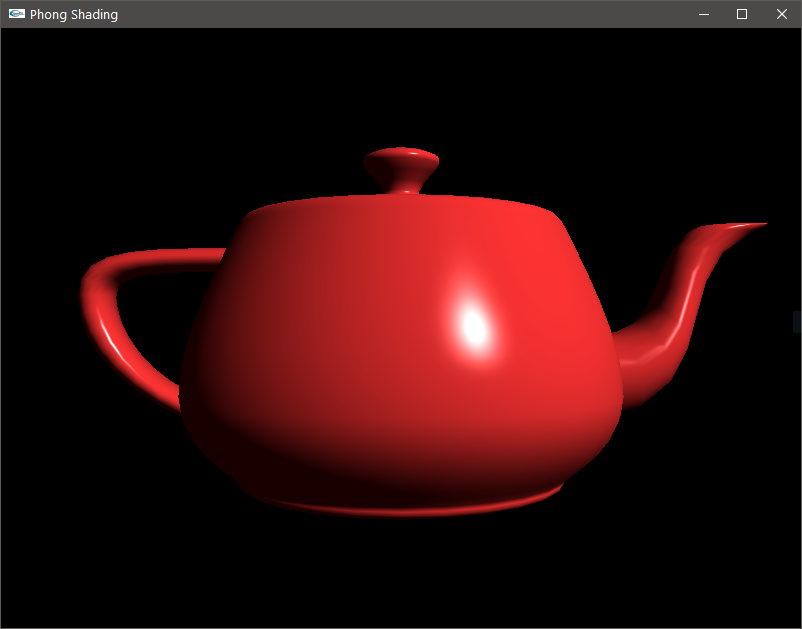
\includegraphics[scale=0.15]{q5-red.png}
        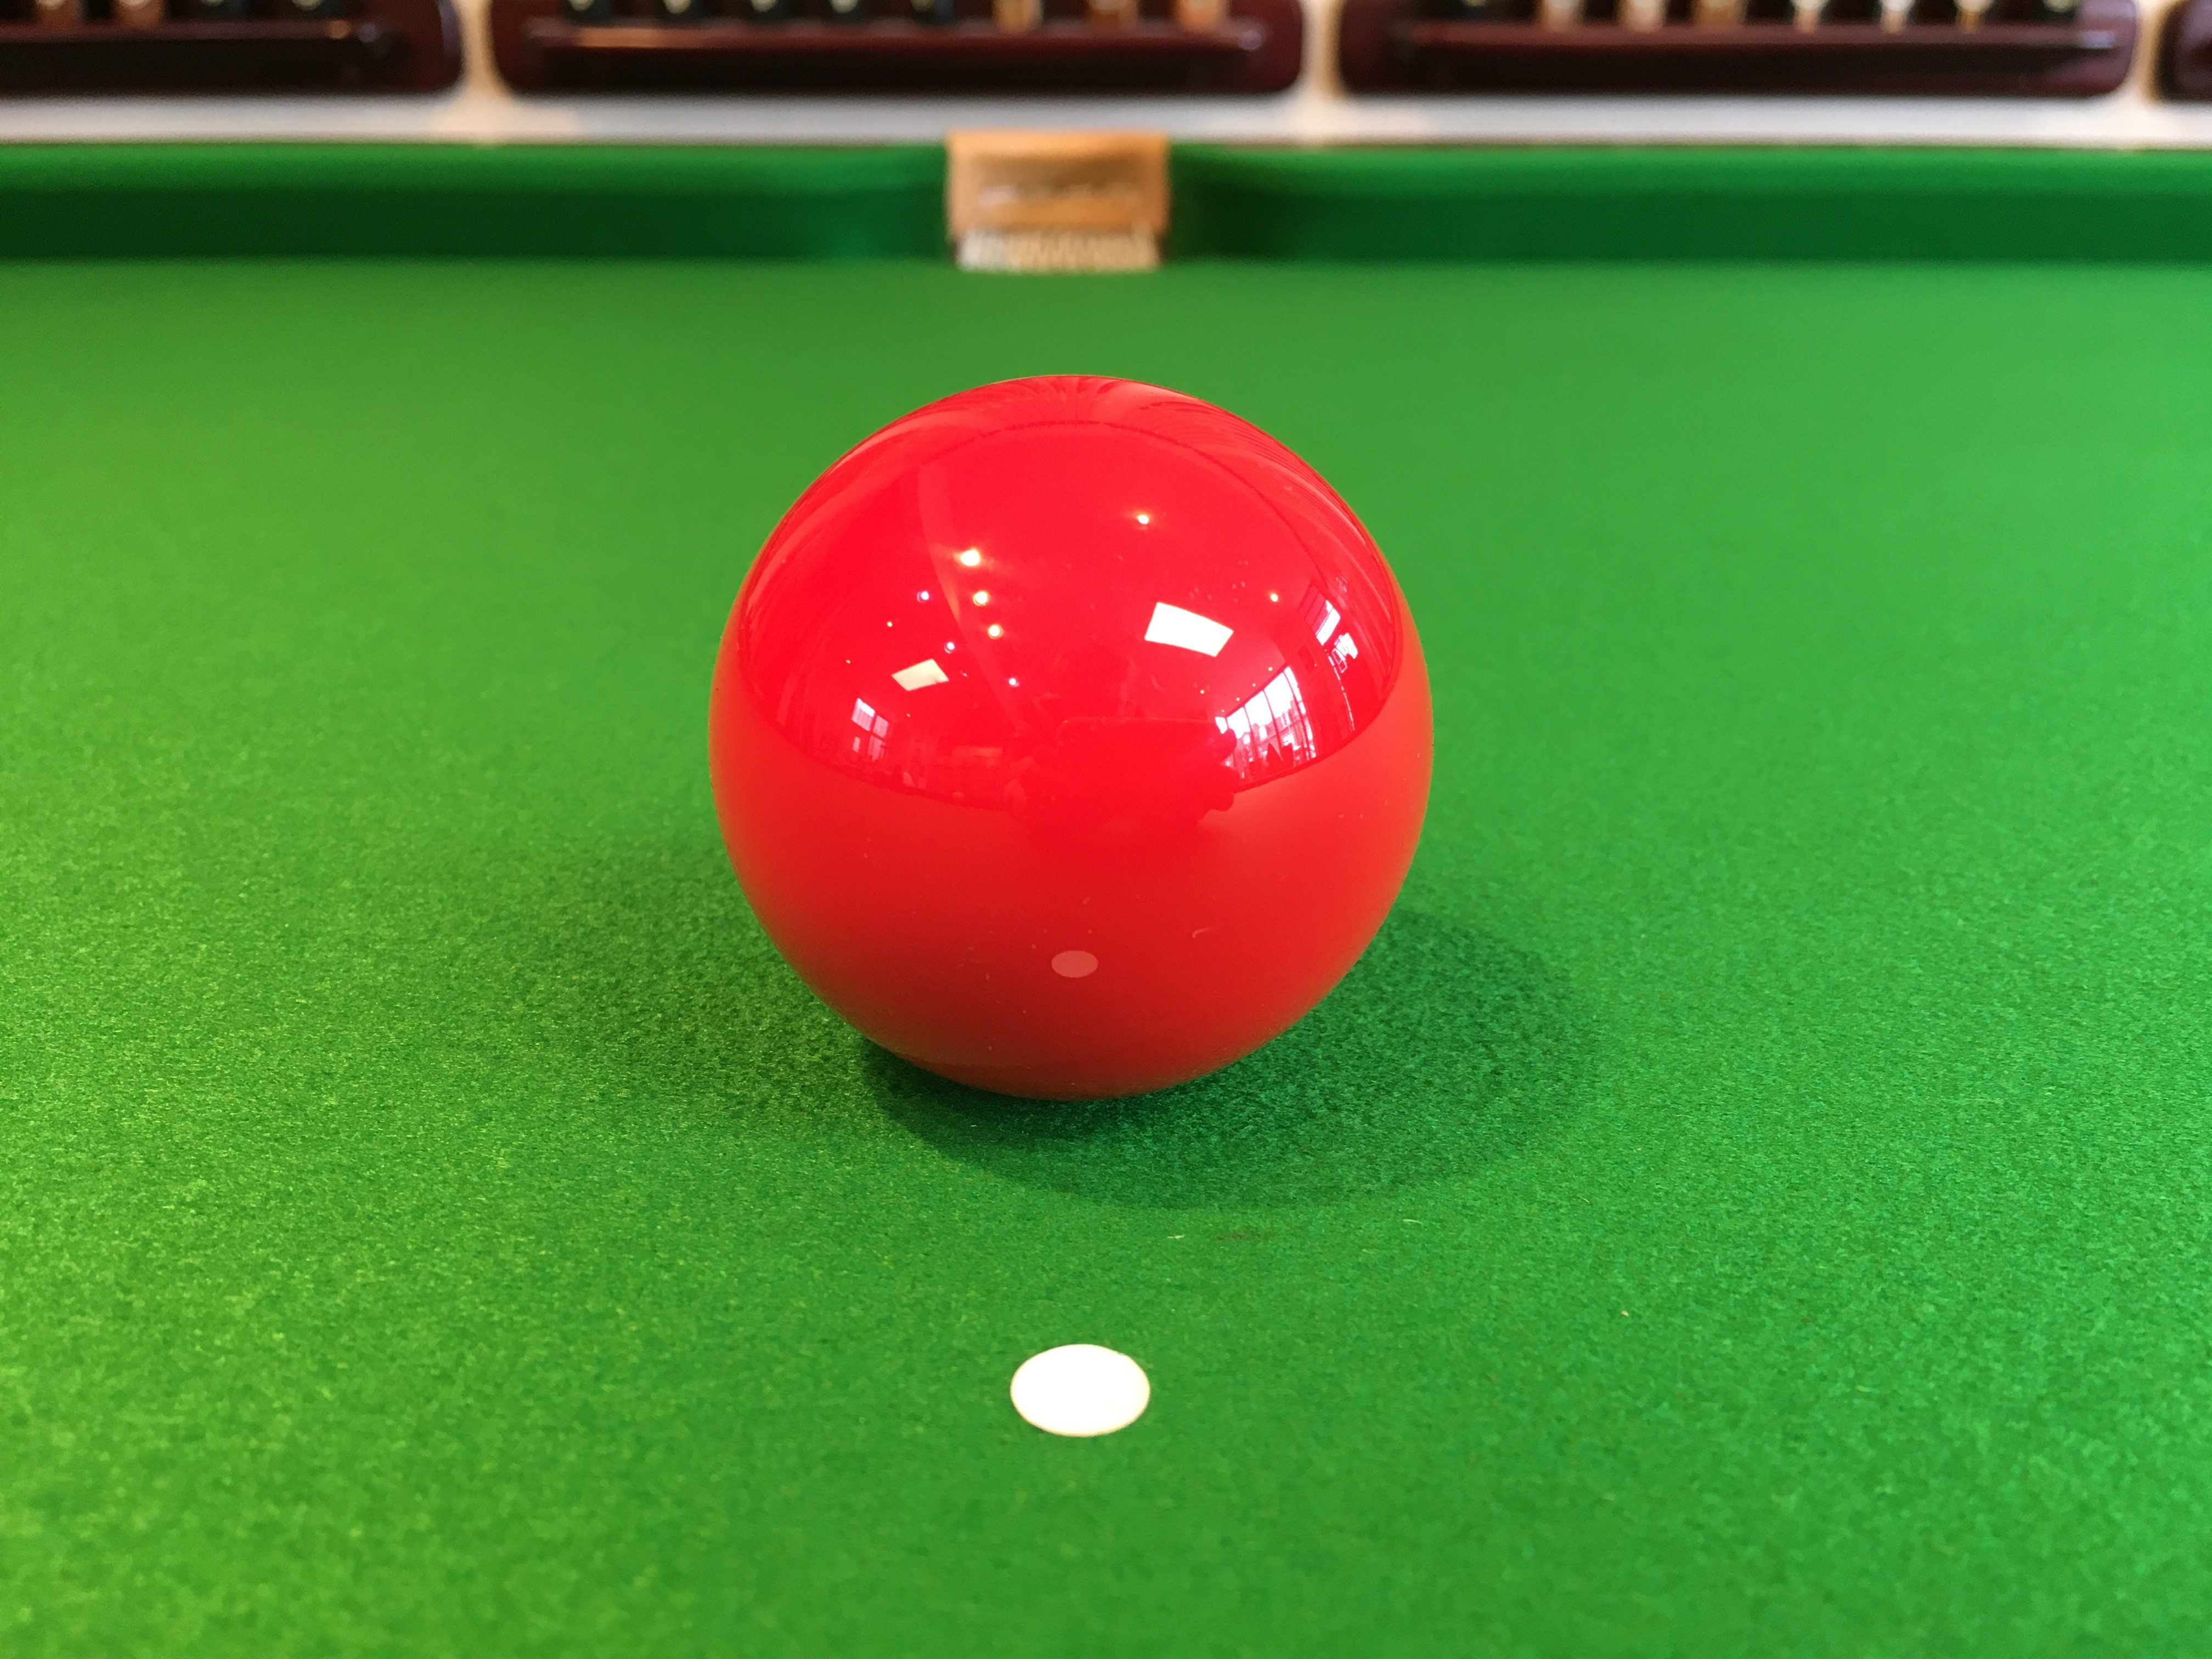
\includegraphics[scale=0.03]{red-billiard.jpg}
    \end{center}

    \begin{enumerate}
        \item $k_d$ = [0.9, 0.2, 0.2]
        \item $k_s$ = [1.0, 1.0, 1.0]
        \item $n$ = 64.0
    \end{enumerate}

\end{frame}

\begin{frame}
    \frametitle{Dry white clay}

    \begin{center}
        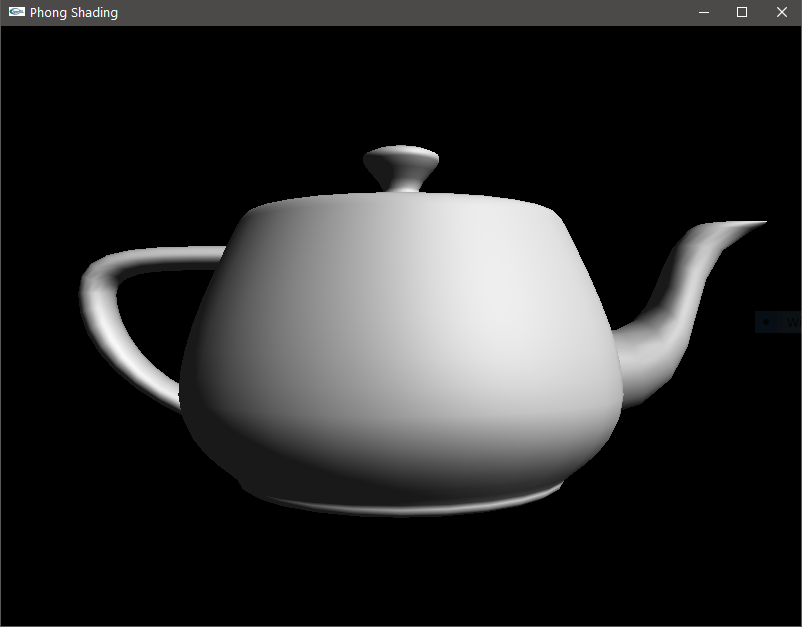
\includegraphics[scale=0.15]{q5-white-clay.png}
        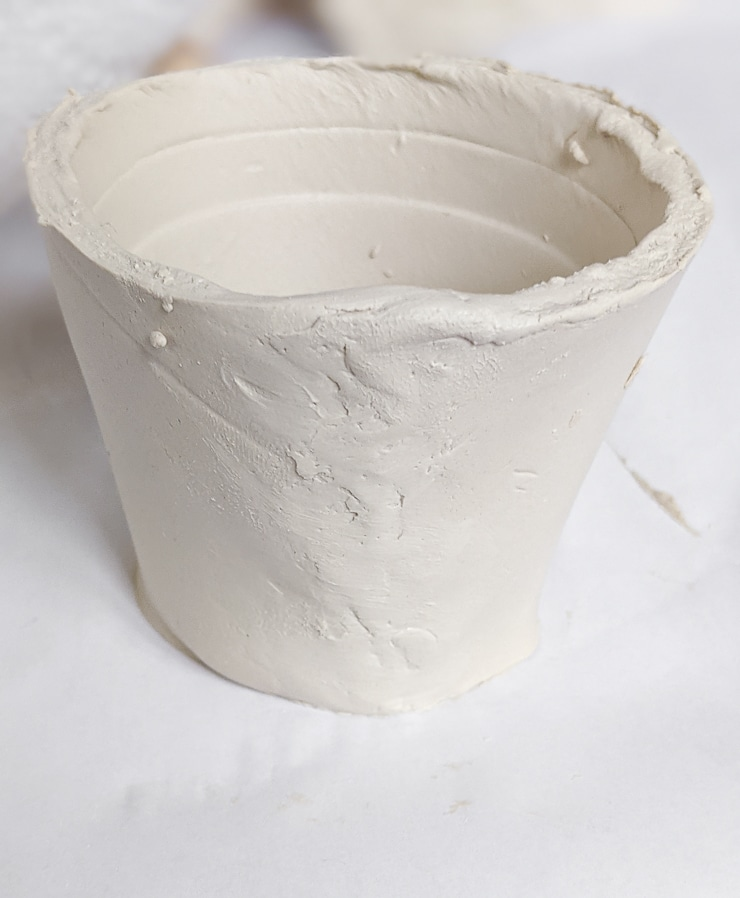
\includegraphics[scale=0.1]{white-clay.jpg}
    \end{center}

    \begin{enumerate}
        \item $k_d$ = [0.8, 0.8, 0.8]
        \item $k_s$ = [0.1, 0.1, 0.1]
        \item $n$ = 1.0
    \end{enumerate}

\end{frame}

\begin{frame}
    \frametitle{Brushed Bronze}

    \begin{center}
        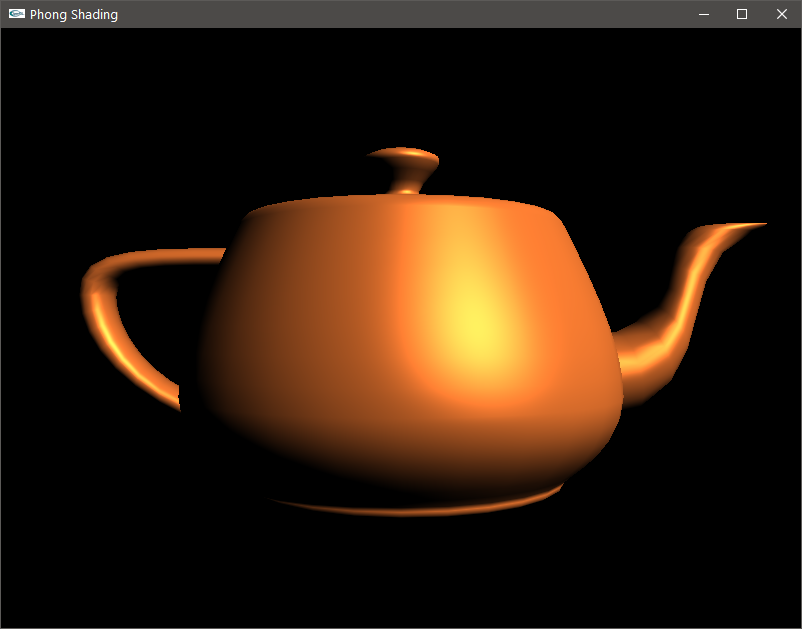
\includegraphics[scale=0.18]{q5-bronze.png}
        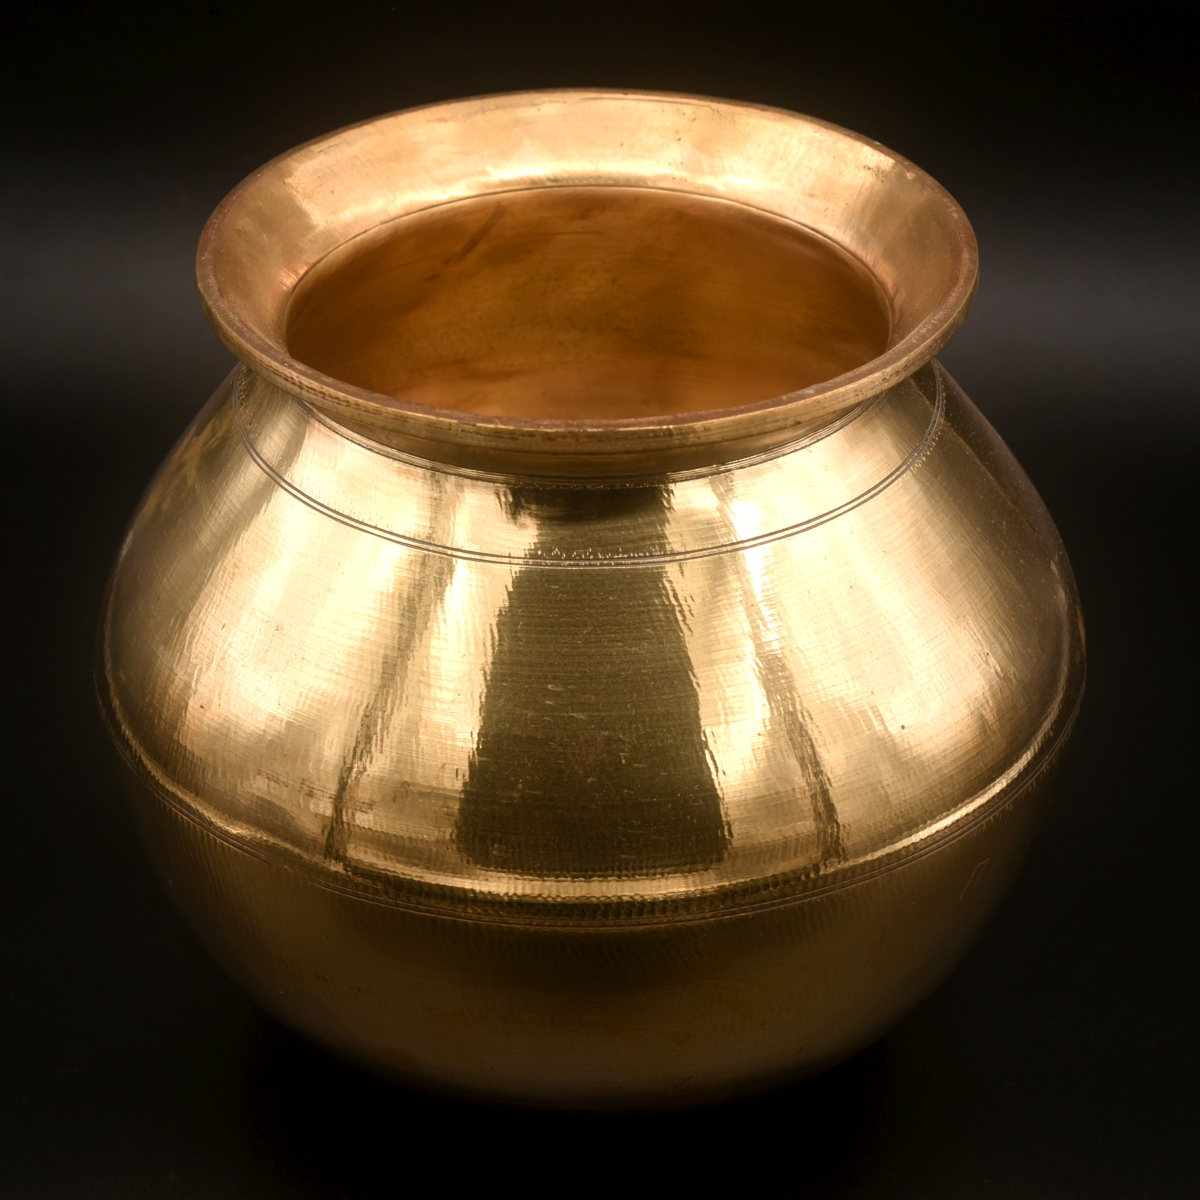
\includegraphics[scale=0.1]{bronze-pot.jpg}
    \end{center}

    \begin{enumerate}
        \item $k_d$ = [1.0, 0.5, 0.2]
        \item $k_s$ = [1.0, 0.5, 0.2]
        \item $n$ = 8.0
    \end{enumerate}

\end{frame}

\begin{frame}
    \frametitle{Points to note}

    \begin{itemize}
        \item If object is completely diffuse: $k_s = [0, 0, 0]$
        \item If object is mostly diffuse: Lower value of $k_s$
        \item Metallic: $k_d = k_s$
        \item Shininess (smaller highlights): Higher $n$
    \end{itemize}

\end{frame}

\section{Question 6}

\begin{frame}
    \frametitle{Question 6}

    Consider a variant of the Phong model, called the Blinn-Phong model, whose computation is 

    \begin{equation*}
        I_\text{Blinn-Phong} = I_a k_a + I_p k_d  (N \cdot L) + I_p k_s (\textcolor{violet}{N \cdot H})^n
    \end{equation*}
    $H$ is called the Half vector and it is the vector exactly in the middle of $L$ and $V$.

\end{frame}

\begin{frame}
    \frametitle{Blinn Phong $H$ vector}

    % \begin{tcolorbox}[colback=teal!5!white] \textcolor{teal}{pollev.com/peixian} \end{tcolorbox}
    % \vspace*{1em}

    Write an expression to compute $H$. Note that $H$ must be a unit vector.

    \vspace*{2em}

\end{frame}

\begin{frame}
    \frametitle{Blinn Phong $H$ Vector}

    \begin{equation*}
        H = \frac{L + V}{|L + V|}
    \end{equation*}

    \begin{center}
        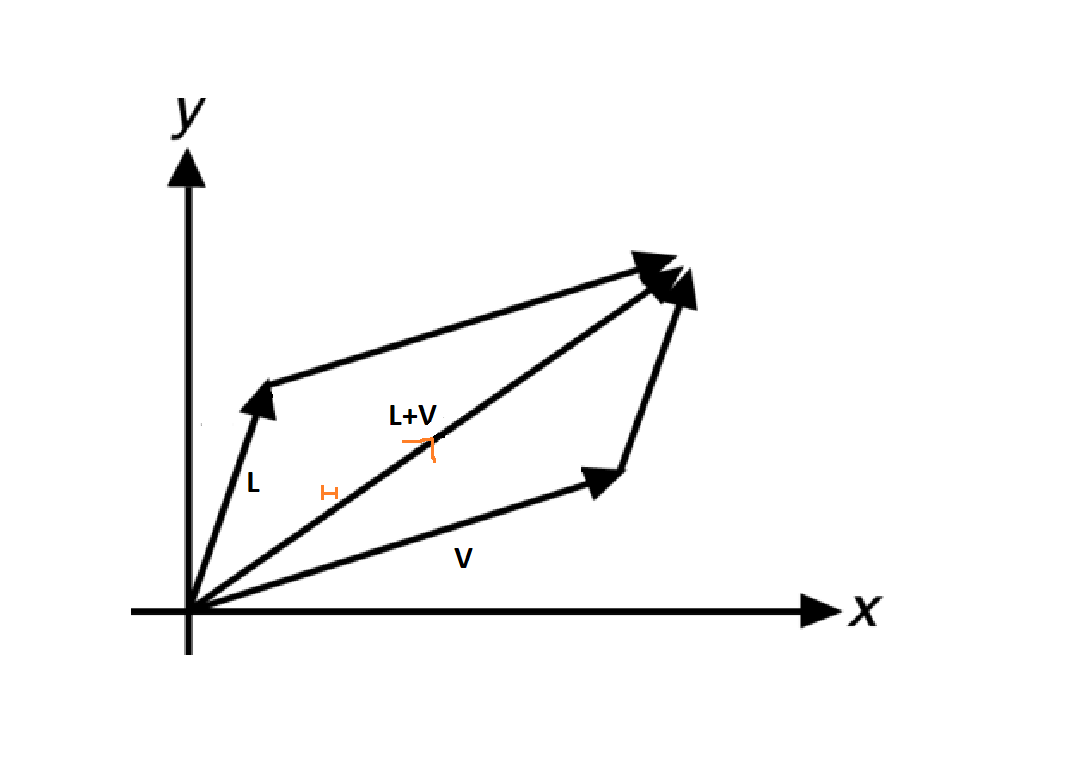
\includegraphics[scale=0.4]{h-vector.png}
    \end{center}

\end{frame}

\begin{frame}
    \frametitle{Blinn Phong vs Phong}

    What is the difference in appearance between a surface rendered using
    Phong model and the same surface rendered using Blinn-Phong model?

    \begin{center}
        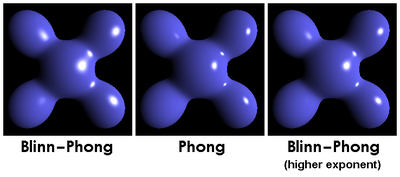
\includegraphics[scale=0.4]{blinnvsphong.png}
    \end{center}

    \begin{tcolorbox}
        The specular highlights from Blinn-Phong model will be relatively larger.
    \end{tcolorbox}

\end{frame}

\begin{frame}
    \frametitle{Computation of specular term}

    Is there an advantage in using $N \cdot H$ over using $R \cdot V$ to compute the specular term? 
    If yes, what is that?

    \begin{center}
        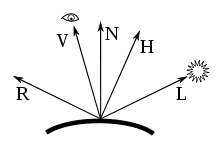
\includegraphics[]{blinn-phong.png}
    \end{center}

\end{frame}

\begin{frame}
    \frametitle{Faster computation of specular term}

    What happens when \textbf{light source} and \textbf{viewer} are very far away?

    \begin{center}
        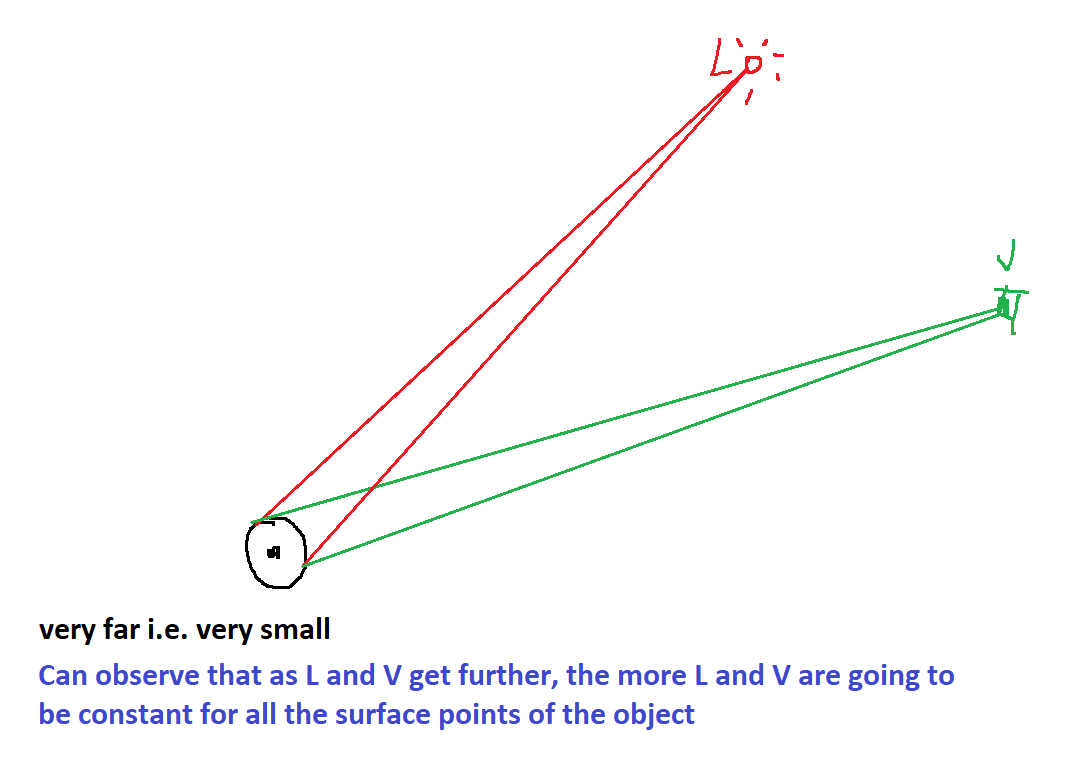
\includegraphics[scale=0.5]{NHvsRV.png}
    \end{center}

\end{frame}

\begin{frame}
    \frametitle{$H$ vector}

    \begin{itemize}
        \item If $L$, $V$ are far, then $L$, $V$ are mostly constant across surface points
        \item Value of $H$ can be cached
        \item Unlike for $R$, which must be recomputed per surface point (different $N$ per surface point).
        \item Hence computation of $N \cdot H$ is faster than $R \cdot V$.
    \end{itemize}

\end{frame}

\section{Question 7}

\begin{frame}
    \frametitle{Question 7}

    A retroreflector reflects most of the light back in the incident direction. 
    For example, most road signs are retroreflectors. 

    \vspace*{1em}

    Suppose we have a retroreflective material that behaves very similarly to a Phong material,
    with a diffuse and specular component, except that the specular reflection is \textbf{centered 
    about the direction of the incident light}.

    \vspace*{1em}

\end{frame}

\begin{frame}
    \frametitle{Question 7}

    % \begin{tcolorbox}[colback=teal!5!white] \textcolor{teal}{pollev.com/peixian} \end{tcolorbox}
    % \vspace*{1em}

    \begin{tcolorbox}
        Suppose we have a retroreflective material that behaves very similarly to a Phong material,
        with a diffuse and specular component, except that the specular reflection is \textbf{centered 
        about the direction of the incident light}.
    \end{tcolorbox}

    \vspace*{1em}

    Modify the Phong Illumination Equation to model this retroreflective reflection. 

    \begin{equation*}
        I_\text{Phong} = I_a k_a + I_p k_d  (N \cdot L) + I_p k_s (R \cdot V)^n
    \end{equation*}

\end{frame}

\begin{frame}
    \frametitle{Question 7}

    We modify only the specular term of the original PIE to $I_p k_s (L \cdot V)^n$.

    \begin{tcolorbox}
        \begin{equation*}
            I_\text{Retro-PIE} = I_a k_a + I_p k_d  (N \cdot L) + I_p k_s (L \cdot V)^n
        \end{equation*}
        \textbf{centered about the direction of the incident light}.
    \end{tcolorbox}

\end{frame}

\begin{frame}
    \frametitle{Retroreflectors in real life}

    \begin{center}
        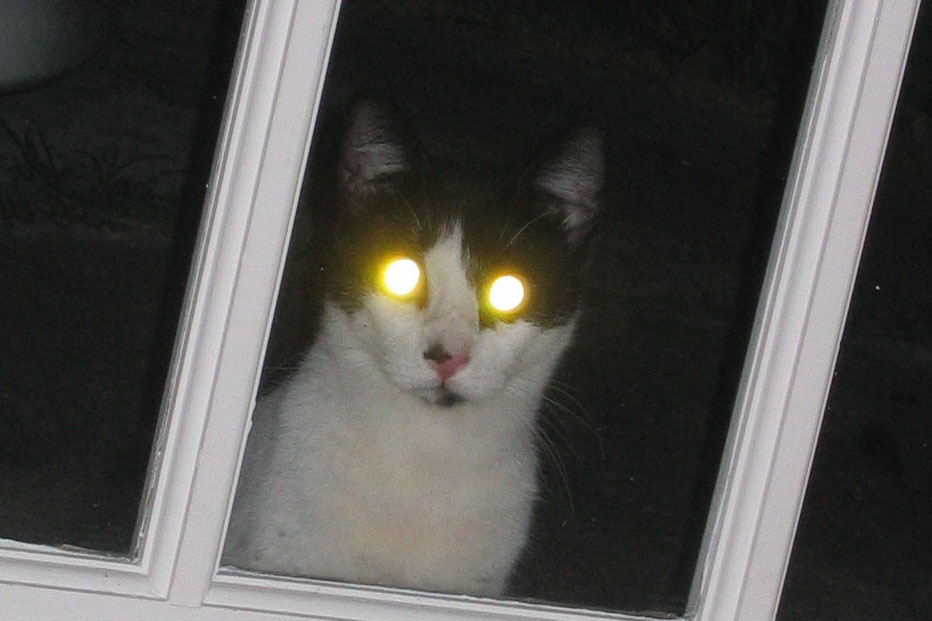
\includegraphics[scale=0.6]{cat-eye.jpg}
    \end{center}

\end{frame}

\begin{frame}
    \frametitle{Retroreflectors in real life}

    \begin{center}
        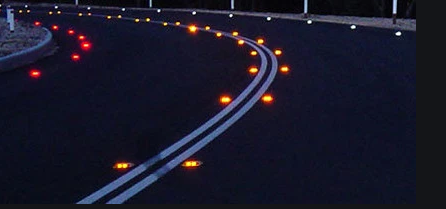
\includegraphics[scale=0.7]{road-cat-eye.png}
    \end{center}

\end{frame}

\begin{frame}
    \frametitle{Question 8}

    How is Phong Shading computationally more expensive than Gouraud Shading in general?

\end{frame}

\begin{frame}
    \frametitle{Phong vs Gouraud shading}

    \textbf{Phong Shading}: requires lighting computation at \textit{every fragment}\\
    \textbf{Gouraud Shading}: requires lighting computation at \textit{every vertex}, which resulting color is interpolated\\

    \begin{tcolorbox}
        \# Vertices $<<$ \# Fragments
    \end{tcolorbox}

\end{frame}

\begin{frame}[plain,standout]
    \AlegreyaExtraBold \LARGE
    Attendance taking
\end{frame}

\ThankYou
\begin{frame}[plain,standout]
    Thanks! Get the slides here after the tutorial.\\
    \vspace{2em}
    \scalebox{3}{\faGithub}\par\bigskip
    \url{https://trxe.github.io/cs3241-notes}
\end{frame}

\end{document}